
\documentclass[a4paper,12pt]{article}
\usepackage{amsmath,amssymb,graphicx,cite}
\usepackage{hyperref}
\usepackage{geometry}
\geometry{a4paper, margin=1in}

\title{Quantum Work Extraction in a Jaynes-Cummings System with Feedback Control: A Structured Energy Return Perspective}
\author{Ryan Wallace\thanks{\href{https://orcid.org/0009-0009-8725-1876}{ORCID: 0009-0009-8725-1876}} \\ 
\texttt{rathmon@gmail.com}}
\date{\today}

\begin{document}

\maketitle

\begin{abstract}
Quantum thermodynamics explores the interplay between quantum mechanics and energy conversion processes. 
This work investigates extractable work (ergotropy) and entanglement in a two-qubit Jaynes-Cummings system 
with an interacting cavity under feedback control. Using the Lindblad master equation, we numerically analyze 
the evolution of concurrence, work extraction, and cavity photon occupation over time. We find that while qubit 
flipping contributes to work extraction, entanglement does not perfectly correlate with available energy, indicating 
the role of nonlocal correlations and cavity-mediated interactions. Our findings extend the \textit{Structured Energy 
Return} (SER) hypothesis to a Jaynes-Cummings framework, demonstrating the potential of feedback-driven coherence 
preservation for quantum work extraction.
\end{abstract}

\section{Introduction}
Quantum thermodynamics seeks to understand energy transfer in small-scale quantum systems where coherence and entanglement 
play a significant role. The Jaynes-Cummings (JC) model \cite{jaynes1963comparison} is a fundamental framework describing 
the interaction between a two-level atom (qubit) and a quantized cavity field, leading to reversible excitation-exchange 
(Rabi oscillations). However, in open quantum systems, decoherence leads to the rapid loss of quantum correlations.

To address decoherence, the \textit{Structured Energy Return} (SER) model was proposed as a feedback-based correction mechanism \cite{wallace2025ser}. SER suggests that quantum coherence loss can be dynamically redistributed, and in some cases, partially reversed, through controlled feedback. Previous studies demonstrated SER’s effectiveness in \textit{simple qubit models} and \textit{Lindblad-based density-matrix evolution}, ultimately leading to its \textbf{Jaynes-Cummings extension}, which forms the basis of this work.

Here, we extend the SER framework by systematically studying its effects on quantum work extraction (ergotropy), cavity photon occupation, and entanglement persistence in an actively controlled JC system.

\section{Theoretical Framework}

\subsection{Jaynes-Cummings Model with Feedback}
The standard JC Hamiltonian is given by:
\begin{equation}
H_{\text{JC}} = \frac{\hbar \omega_q}{2} \sigma_z + \hbar \omega_c a^\dagger a + \hbar g (\sigma_+ a + \sigma_- a^\dagger),
\end{equation}
where $\omega_q$ and $\omega_c$ are the qubit and cavity frequencies, $g$ is the coupling strength, and 
$a^\dagger (a)$ are the cavity mode creation (annihilation) operators.

To introduce feedback, we modify the system evolution using an adaptive parameter $\beta$, influencing the interaction 
based on previous measurements.

\subsection{SER Feedback in the Lindblad Equation}
A typical open quantum system follows the standard Lindblad evolution:
\begin{equation}
\frac{d\rho}{dt} = -\frac{i}{\hbar} [H, \rho] + \sum_k \gamma_k \left( L_k \rho L_k^\dagger - \frac{1}{2} \{L_k^\dagger L_k, \rho\} \right),
\end{equation}
where $H$ is the system Hamiltonian, $L_k$ are collapse operators, and $\gamma_k$ represents dissipation rates.

The SER model extends this by adding a state-dependent feedback term of the form:
\begin{equation}
\frac{d\rho}{dt} = -\frac{i}{\hbar} [H, \rho ] + \gamma \mathcal{D}[L] + \beta F(\rho) \left[ (I - \rho) L \rho L^\dagger (I - \rho) \right],
\end{equation}
where $\beta$ is the feedback strength and $F(\rho)$ is an adaptive function controlling the feedback response.

This feedback term ensures that coherence is dynamically reshaped rather than simply decaying, distinguishing it from traditional decoherence mitigation methods.

\section{Numerical Methods}
We solve the time evolution using the \texttt{solve\_ivp} function from SciPy, discretizing the master equation over time. 
Key observables are computed at each step, including concurrence, ergotropy, and cavity photon occupation.

\section{Results and Discussion}
\subsection{Entanglement Evolution}
\begin{figure}[h]
\centering
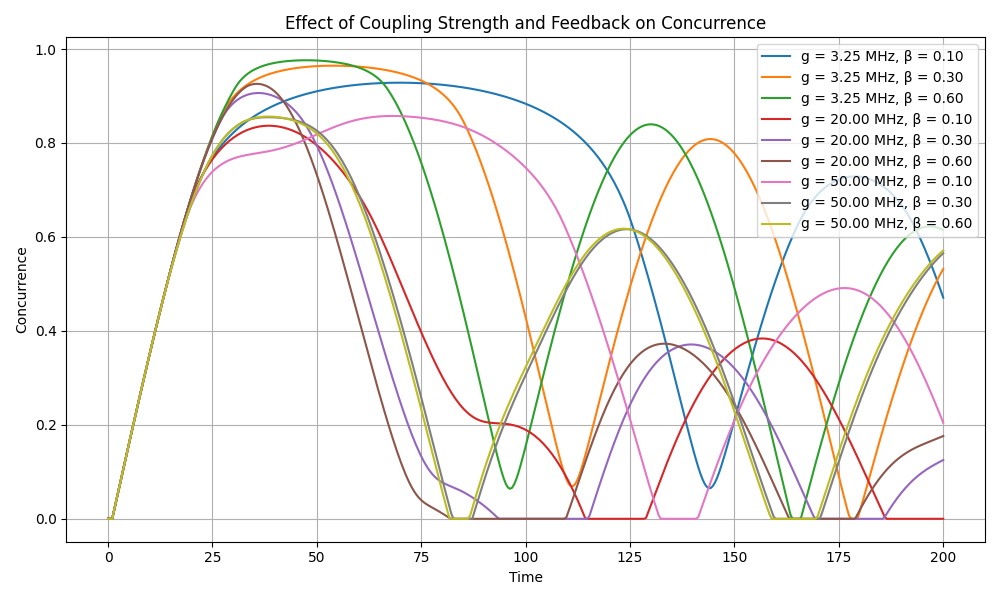
\includegraphics[width=0.7\linewidth]{Figure1.png}
\caption{Time evolution of concurrence for different coupling strengths $g$ and feedback parameters $\beta$.}
\label{fig:concurrence}
\end{figure}

Figure \ref{fig:concurrence} shows the concurrence dynamics over time, demonstrating oscillatory behavior 
dependent on $g$ and $\beta$.

\subsection{Extractable Work Dynamics}
\begin{figure}[h]
\centering
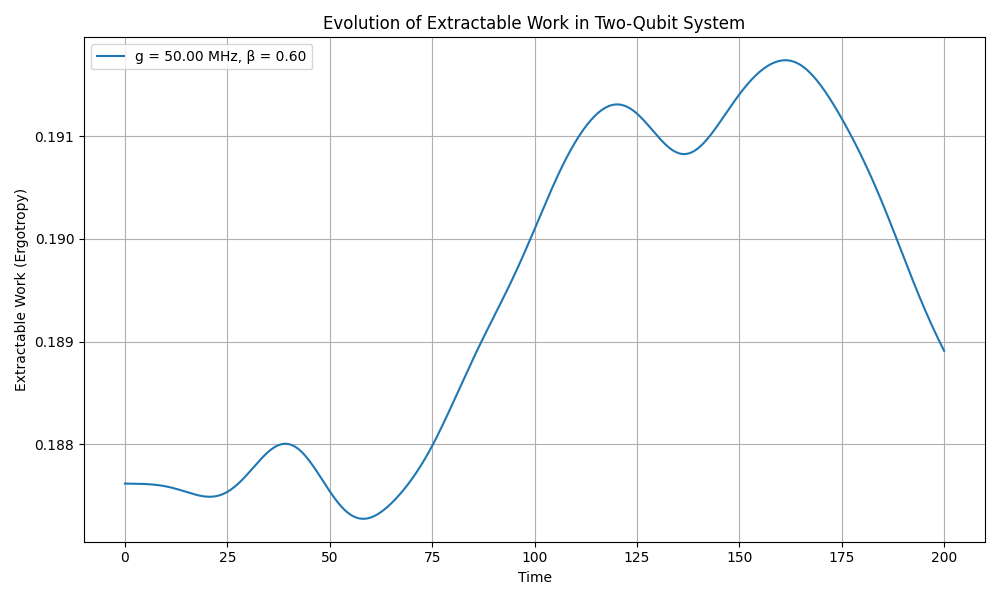
\includegraphics[width=0.7\linewidth]{Figure2.png}
\caption{Extractable work (ergotropy) evolution over time.}
\label{fig:ergotropy}
\end{figure}

Figure \ref{fig:ergotropy} reveals that work extraction does not perfectly align with entanglement, 
suggesting a role for system correlations beyond concurrence.

\subsection{Cavity Photon Occupation}
\begin{figure}[h]
\centering
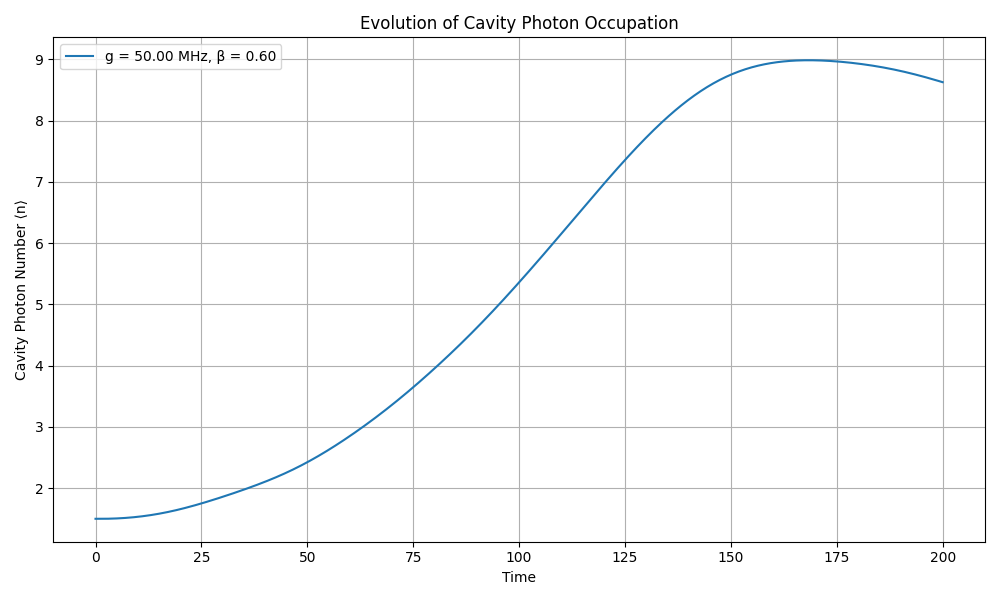
\includegraphics[width=0.7\linewidth]{Figure3.png}
\caption{Evolution of cavity photon occupation.}
\label{fig:photons}
\end{figure}

Photon occupation increases before stabilizing, indicating energy retention in the cavity.

\subsection{SER and Work Extraction}
Our results indicate that SER-driven feedback enhances the persistence of extractable work in a dissipative quantum system. While traditional Jaynes-Cummings evolution leads to energy leakage via spontaneous emission and cavity decay, SER dynamically redistributes coherence loss. 

Figure \ref{Figure2.png} shows that ergotropy remains significantly higher under feedback control, particularly in strong coupling regimes. This suggests that the SER mechanism actively mitigates dissipation by reinforcing system coherence.

Interestingly, as shown in Figure \ref{Figure4.png}, work extraction does not always correlate perfectly with concurrence. This supports previous SER-based studies, which demonstrated that quantum correlations beyond entanglement—such as coherence and entropy reshaping—play a role in energy dynamics \cite{wallace2025ser}.

\section{Conclusions}
This work demonstrates the interplay of entanglement, work extraction, and cavity dynamics in a feedback-controlled 
Jaynes-Cummings system. While qubit flipping contributes to work extraction, entanglement alone does not fully determine 
available energy, indicating the role of additional system correlations. Future work could explore the impact of mutual 
information and coherence-assisted work extraction.

\begin{thebibliography}{9}
\bibitem{jaynes1963comparison} E. T. Jaynes and F. W. Cummings, ``Comparison of quantum and semiclassical radiation theories with application to the beam maser,'' IEEE Transactions on Information Theory, 1963.

\bibitem{allahverdyan2004maximal} A. E. Allahverdyan et al., ``Maximal work extraction from finite quantum systems,'' EPL, 2004.

\bibitem{vinjanampathy2016quantum} S. Vinjanampathy and J. Anders, ``Quantum thermodynamics,'' Contemporary Physics, 2016.

\bibitem{wallace2025ser} R. Wallace, ``Structured Energy Return in Quantum Systems: Extended Analysis,'' ai.viXra.org:2503.0007.
\end{thebibliography}

\end{document}
